\section{Косинусный закон преломления}
\begin{frame}[plain, noframenumbering]
    \begin{center}
        \Huge
        Косинусный закон преломления
    \end{center}
\end{frame}

\begin{frame}\frametitle{Косинусный закон преломления}


\qq Преломление по закону косинусов: 
\begin{itemize}
\item[1.] Выполнено соотношение $n_i \cos \theta_i = n_j \cos \theta_j $, где $\theta_i, \theta_j \in [0,\frac{\pi}{2} ]$ -- углы, которые образуют падающий и преломленный лучи с нормалью к кривой $C$, если $\theta_i$ и $\theta_j$ корректно определены.
\item[2.] Если косинус преломленного оказывается больше 1, происходит полное внутреннее отражение по закону <<угол падения равен углу отражения>>.
\item[3.] В предыдущих двух пунктах  соседние отрезки траектории с общей точкой на кривой $C$ лежат по разные стороны от нормали к кривой.
\item[4.] Если $n_i > n_j$ и материальная точка, двигаясь в области $\Omega_j$, достигает кривой $C$, причем $\theta_j = 0$, тогда $\cos \theta_i = \frac{n_j}{n_i}$ и материальная точка продолжает движение в области $\Omega_i$ вдоль любого из двух возможных направлений, образующих угол $\theta_i$ с нормалью к кривой $C$.
\item[5.] Аналогично при $n_i < n_j$.
\end{itemize}
\end{frame}
\note{
    Этот текст будет виден только если его отображение включено
    в~файле \textbf{Presentation/setup}.
    Для раздельного вывода презентации и заметок на~разные экраны (как
    в~impress или powerpoint) можно использовать программу
    \textit{pdf-presenter-console}.
}

\subsection{Не нумерованные}


\begin{frame}\frametitle{Косинусный закон преломления}


\begin{figure}
\begin{minipage}[t]{0.3\linewidth}
        \centering
        \includegraphics[width=3.5cm]{./portraits domain.png}
        \caption{Две среды.}
    \end{minipage}
    \hfill
    \begin{minipage}[t]{0.57\linewidth}
        \centering
        \includegraphics[scale=0.23]{./phase portraits/better cosine portrait.jpg}
        \caption{Фазовый портрет для преломления по закону косинусов.}
    \end{minipage}
\end{figure}
\end{frame}
\note[itemize]{
    \item Тезис 1
    \item Тезис 2
    \item Тезис 3
}

\begin{frame}\frametitle{Косинусный закон преломления --- простой случай}

\qq Граница сред --- софокусный эллипс, на границе сред преломление по косинусному закону

\begin{figure}[!htb]
\centering
\includegraphics[width=7cm]{./portraits domain 2.png}
%    \caption{Две среды, закон Снеллиуса.}
\end{figure}
\end{frame}
\note[itemize]{

}

\begin{frame}\frametitle{Косинусный закон преломления --- простой случай}


\begin{mytheorem}

Имеет место формула, связывающая параметры каустик (софокусных квадрик) до и после преломления:
$$n_1^2  \cdot ( \Lambda(\mathbf{x}, \mathbf{v}) - \lambda_0 )= n_2^2 \cdot (\Lambda(\mathbf{x}, \mathbf{w}) - \lambda_0).$$
В ней участвуют:
 параметр $\lambda_0$ преломляющей квадрики и коэффициенты $n_1, n_2$ <<оптической>> плотности двух сред, \\$\mathbf{x}$ --- точка преломления, \\$\mathbf{v}$ и $\mathbf{w}$ --- векторы скоростей до и после преломления.

$\Lambda(\mathbf{x}, \mathbf{v})$ --- функция, вычисляющая касательную квадрику к прямой, проходящей через точку $\mathbf{x}$ вдоль вектора $\mathbf{v}$.
\end{mytheorem}

\end{frame}

\begin{frame}
\center\LARGE Первый интеграл
\end{frame}


\begin{frame}\frametitle{Интеграл без ветвления}

\qq Случай легко обобщается на несколько непересекающихся квадрик

\begin{figure}[!htb]
    \centering
    \includegraphics[width=0.45\textwidth]{part11/multiple ellipses.pdf}
    \includegraphics[width=0.35\textwidth]{part11/multiple hyperbolas.pdf}  
    \caption{Варианты взаимного расположения областей $\Omega_1, \ldots, \Omega_k$.}
\end{figure}
%\end{frame}
%
%%Здесь и далее коэффициент плотности в области $\Omega_j$ обозначим через $n_j$.
%\begin{frame}\frametitle{Интеграл без ветвления}


\qq Определим функцию $\Xi(\mathbf{x}, \mathbf{v})$ по формуле: 
\begin{equation*}
\Xi(\mathbf{x}, \mathbf{v}) = \left[
\begin{array}{ll}
    \Lambda(\mathbf{x}, \mathbf{v}) n_1^2, &  \text{ для } \mathbf{x} \in \Omega_1 
    \\
    \Lambda(\mathbf{x}, \mathbf{v}) n_p^2 + 
    \sum_{j=1}^{p-1} \lambda_j(n_j^2-n_{j+1}^2), & \text{ для } \mathbf{x} \in \Omega_p \text{ и } 1 < p \leq k. 
\end{array}
\right.
\end{equation*}

\begin{mytheorem}
Функция $\Xi(\mathbf{x}, \mathbf{v})$ является постоянной на траекториях бильярда в областях рассматриваемого вида с  преломлением по закону косинусов.
\end{mytheorem}
\end{frame}


\begin{frame}\frametitle{Интеграл с ветвлением (1 точка ветвления)}

\qq 
Внутренность эллипса разделена на области дугами софокусных квадрик таким образом, что имеются всего 1 точка их пересечения, которую обозначим $A$. Например,
\begin{figure}[!htb]
\centering
\includegraphics[width=3cm]{part11/img2.pdf}
\caption{Взаимное расположение областей $\Omega_1,\ldots,\Omega_4$}
\label{fig:xi_is_integral}
\end{figure}

\qq Общая часть границы $\Omega_1 \cup \Omega_4$ и $\Omega_2 \cup \Omega_3$ --- дуга софокусной квадрики с параметром $\lambda_1$, а общая часть границы $\Omega_1 \cup \Omega_2$ и $\Omega_3 \cup \Omega_4$ --- дуга софокусной квадрики с параметром $\lambda_2$.
\end{frame}

\begin{frame}\frametitle{Интеграл с ветвлением (1 точка ветвления)}
\qq Введем \underline{индекс ветвления} в точке $A$ по формуле \begin{align*}
\gamma_A = (\lambda_1 - \lambda_2) ( n_1^2 - n_2^2 + n_3^2 - n_4^2).
\end{align*}



\qq Определим вспомогательную функцию $\widetilde{\Xi}(\mathbf{x}, \mathbf{v})$ 
\begin{equation*}
\widetilde{\Xi}(\mathbf{x}, \mathbf{v}) = \left[
\begin{array}{ll}
    \Lambda(\mathbf{x}, \mathbf{v}) n_1^2, &  \text{ для } \mathbf{x} \in \Omega_1 
    \\
    \Lambda(\mathbf{x}, \mathbf{v}) n_p^2 + 
    \sum_{j=1}^{p-1} \lambda_{\sigma(j)}(n_j^2-n_{j+1}^2), \!\!\!& \text{ для } \mathbf{x} \in \Omega_p \text{ и } 1 < p \leq 4,
\end{array}
\right.
\end{equation*}
где $\sigma(j)$ -- номер квадрики, разделяющей $\Omega_j$ и $\Omega_{j+1}$.

\qq Она почти подходит на роль дополнительного интеграла: \\
она постоянна на любом звене траектории, не пересекающем дугу $\partial \Omega_1  \cap \partial  \Omega_4$. \\Однако, на любой бильярдной траектории, пересекающей эту дугу, функция $\widetilde{\Xi}(\mathbf{x}, \mathbf{v})$ испытывает \underline{один и тот же скачок}, равный индексу ветвления $\gamma_A$. 
\end{frame}

\begin{frame}\frametitle{Интеграл с ветвлением (1 точка ветвления)}
\qq Определим функцию $\Xi(\mathbf{x}, \mathbf{v})$ со значениями в $S^1= \mathbb{R}/\gamma_A \mathbb{Z}$ по формуле $$\Xi(\mathbf{x}, \mathbf{v}) = \widetilde{\Xi}(\mathbf{x}, \mathbf{v}) \mod \gamma_A.$$

\begin{mytheorem}
Для биллиарда с  разбиением на области  

\begin{figure}[!htb]
\centering
\includegraphics[width=3cm]{part11/img2.pdf}
\end{figure}
с преломлением по закону косинусов\\
функция $\Xi(\mathbf{x}, \mathbf{v})$ является постоянной на траекториях.
\end{mytheorem}
\end{frame}

\begin{frame}
\frametitle{Интеграл с ветвлением (2 точки ветвления)}

\qq Разбиение на области
\begin{figure}[!htb]
    \centering
     \includegraphics[width=0.25\textwidth]{part11/img3.pdf}
\caption{Взаимное расположение областей $\Omega_1,\ldots,\Omega_4$}
\end{figure} 

\qq Индексы  ветвления в точках $A_1, A_2$:
$$\gamma_{A_1} = \lambda_2(n_1^2 - n_4^2) + \lambda_1(n_4^2-n_3^2) + \lambda_2(n_3^2-n_2^2) + \lambda_1(n_2^2-n_4^2)% = (\lambda_2 - \lambda_1) ( n_1^2 - n_2^2 + n_3^2 - n_4^2).
$$
$$\gamma_{A_2} = \lambda_1(n_1^2 - n_2^2) + \lambda_2(n_2^2-n_3^2) + \lambda_1(n_3^2-n_4^2) + \lambda_2(n_4^2-n_1^2) %= (\lambda_1 - \lambda_2) ( n_1^2 - n_2^2 + n_3^2 - n_4^2).
$$

\qq Заметим, что $$\gamma_{A_1} = -\gamma_{A_2}.$$
\end{frame}

\begin{frame}
\frametitle{Интеграл с ветвлением (2 точки ветвления)}
\qq
Определим  фукцию 
$\Xi(\mathbf{x}, \mathbf{v})$ по модулю $\gamma_{A_1}$  по формуле $$\Xi(\mathbf{x}, \mathbf{v}) = \widetilde{\Xi}(\mathbf{x}, \mathbf{v}) \mod \gamma_{A_1},$$
где 
\begin{equation*}
\widetilde{\Xi}(\mathbf{x}, \mathbf{v}) = \left[
\begin{array}{ll}
    \Lambda(\mathbf{x}, \mathbf{v}) n_1^2, &  \text{ для } \mathbf{x} \in \Omega_1 
    \\
    \Lambda(\mathbf{x}, \mathbf{v}) n_p^2 + 
    \sum_{j=1}^{p-1} \lambda_{\sigma(j)}(n_j^2-n_{j+1}^2), & \text{ для } \mathbf{x} \in \Omega_p, 1 < p \leq 4. 
\end{array}
\right.
\end{equation*}

\begin{mytheorem}
Функция $\Xi(\mathbf{x}, \mathbf{v})$ является первым интегралом.
\end{mytheorem}
\end{frame}

\begin{frame}\frametitle{Интеграл с ветвлением  (2 точки ветвления)}


\begin{figure}[!h]
    \centering
     \includegraphics[width=0.4\textwidth]{part11/img4.pdf}
\end{figure}

в точках $A_1$, $A_2$ задаются формулами:
\qq Индексы ветвления  имеют вид
$$\gamma_{A_1} = (\lambda_3 - \lambda_1)(n_2^2 - n_5^2 + n_6^2 - n_3^2),$$
$$\gamma_{A_2} = (\lambda_3 - \lambda_2)(n_1^2 - n_4^2 + n_5^2 - n_2^2).$$

\qq В зависимости от значений параметров отношение $\dfrac{\gamma_{A_1}}{\gamma_{A_2}}$ может быть как рациональным, так и иррациональным.
\end{frame}


\begin{frame}\frametitle{Интеграл с ветвлением --- общий принцип}

\qq
Для каждой точки пересечения $A_i, i=1,\ldots,m$, определен индекс ветвления $\gamma_{A_i}$. Тогда определен первый  интеграл   $\Xi(\mathbf{x}, \mathbf{v})$ со значениями в $\mathbb{R}/(\gamma_{A_1} \mathbb{Z}+ \ldots + \gamma_{A_m} \mathbb{Z})$. 

\qq Если $\gamma_{A_i}$ соизмеримы, то $\mathbb{R}/(\gamma_{A_1} \mathbb{Z}+ \ldots + \gamma_{A_m} \mathbb{Z}) = S^1$. 

\qq Если же среди $\gamma_{A_i}$ есть пара с иррациональной дробью $\dfrac{\gamma_{A_i}}{\gamma_{A_j}}$, то подгруппа $\gamma_{A_1} \mathbb{Z}+ \ldots + \gamma_{A_m} \mathbb{Z}$ всюду плотна в $\mathbb{R}$. В этом случае, хотя дополнительный интеграл $\Xi(\mathbf{x}, \mathbf{v})$ корректно определен, но использовать его для разделения траекторий невозможно.
\end{frame}



\begin{frame}
\LARGE\center Задача А
\end{frame}

\begin{frame}\frametitle{Постановка задачи}

\qq Эллипс $\frac{x^2}{a^2} + \frac{y^2}{b^2} =1$
ограничивает область $\Omega$.
Софокусным эллипсом $Q_{\lambda_1}$ , где $0 < \lambda_1 < b^2$, область $\Omega$ разбивается на две части: эллипс $\Omega_{in}$ и кольцо $\Omega_{out}$, см. рисунок.
\begin{figure}[!htb]
\centering
\includegraphics[scale=0.4]{section2/domain_problemA.pdf}
    \caption{Область $\Omega$ для задачи А.}
    \label{fig:sect2_problemA}
\end{figure}

\qq Показатели преломления $n_{out}$ для кольца $\Omega_{out}$ и $n_{in}$ для $\Omega_{in}$.

\qq Задача состоит в том, чтобы для указанной динамической системы описать слоение изоэнергетического трехмерного многообразия  на поверхности уровня первого интеграла $\Xi$.
\end{frame}

\begin{frame}\frametitle{Бифуркационная диаграмма (нестандартная).  $\Xi \mapsto \mathbb{R}^2$}
\qq Перестройки поверхностей $\Xi = \const$ постоянного значения первого интеграла зависят от соотношения между коэффициентами преломления $n_1, n_2$ и параметром  $\lambda_1$ преломляющей квадрики. Мы вводим диаграмму, которая содержит в себе информацию обо всех поверхностях уровня и их перестройках для всех соотношений между $n_1, n_2$ и $\lambda_1$ сразу.

\qq Значению интеграла $\Xi$ поставим в соответствие точку плоскости $\mathbb{R}^2$ по формуле
\begin{equation*}
\Xi \mapsto \alpha(\Xi) = (\alpha_{in}, \alpha_{out} ) = \left( \frac{\Xi}{n_{in}^2}, \frac{\Xi - \lambda_1 (n_{in}^2 - n_{out}^2)}{n_{out}^2} \right) = \left( \left. \Lambda \right|_{\Omega_{in}}, \left. \Lambda \right|_{\Omega_{out}} \right).
\label{XiToLine}
\end{equation*}

\qq Геометрический смысл: по горизонтали откладывается параметр каустики для внутренней части системы, а по вертикали --- во внешнем кольце.
\end{frame}

%\begin{frame}\frametitle{Бифуркационная диаграмма (нестандартная). $Im(\Xi) = L$}
%\qq Для фиксированных $\lambda_1, n_{in}, n_{out}$ точка $\alpha(\Xi)$ лежит на прямой $L$, которая в декартовых координатах $(\alpha_{in}, \alpha_{out})$ задается уравнением
%\begin{equation*}
%\alpha_{out} = \alpha_{in} \left(\frac{n_{in}}{n_{out}}\right)^2 + \lambda_1 \frac{n_{out}^2 - n_{in}^2}{n_{out}^2}.
%\label{eq:L_line}
%\end{equation*}
%\qq $\Xi$ выступает параметром на прямой $L$.
%
%\qq Прямая $L$ проходит через точку $(\lambda_1, \lambda_1)$ и имеет  коэффициент наклона, равный $\frac{n_{in}^2}{n_{out}^2}$. 
%
%%\qq Для фиксированного набора $\lambda_1, \dfrac{n_{in}}{n_{out}}$ интеграл $\Xi$ принимает значения на соответствующей прямой $L$.
%\qq Прямая $L$ однозначно соответствует параметрам $\lambda_1, \dfrac{n_{in}}{n_{out}}$.
%
%\qq При возрастании значения интеграла $\Xi$ соответствующая точка на отрезке прямой двигается направо и вверх.
%}
\begin{frame}\frametitle{Диаграмма и прямая $L$}
\begin{figure}[!htb]
\centering
\includegraphics[width=9cm]{section2/long red line bifurcations.png}
    \caption{Область значений $\Xi$ --- отрезок на красной прямой.}
    \label{fig:sect2_diagramPlusIrregular}
\end{figure}
\end{frame}


\begin{frame}\frametitle{Диаграмма. Разбиение $\mathbb{R}^2$.}
\qq Тип бильярдной траектории определяется диаграммой
\begin{figure}[!htb]
% \minipage{0.35\textwidth}
% \centering
% \includegraphics[scale=0.1]{section2/causticTypesBulletsDiagram.pdf}
%     \caption{Области возможного движения бильярдной траектории.}
%     \label{fig:sect2_causticTypesBulletsDiagram}
% \endminipage\hfill
% \minipage{0.55\textwidth}
\centering
\includegraphics[width=8.5cm]{section2/problemAbifurcations.pdf}
    \caption{Возможные типы каустик в $\Omega_{in}$ и $\Omega_{out}$. Жирным выделены особые значения для $\alpha_{in}$, $\alpha_{out}$.}
    \label{fig:sect2_problemAbifurcations}
% \endminipage\hfill
\end{figure}
\end{frame}






%\begin{frame}
%\qq Параметры  $\alpha_{in}$, $\alpha_{out}$ имеют критические значения $\lambda_1, b^2$ и $a^2$. Соответствующие координатные линии, а также диагональ $\alpha_{in} = \alpha_{out}$, разбивают плоскость на области. Формально эти подобласти определены на следующем слайде.
%\begin{figure}[!htb]
%\centering
%\includegraphics[scale=0.1]{section2/problemA_subdivisions.pdf}
%    % \caption{Подразбиение областей $D_1, \ldots, D_4$.}
%    \label{fig:sect2_problemA_subdivisions}
%\end{figure}
%}
\begin{frame}\frametitle{Неособые поверхности уровня $\Xi=\const$}
\begin{mytheorem} 
Областям $D_i^j$ в плоскости $(\alpha_{in}, \alpha_{out})$ соответствуют следующие поверхности $\Xi = \const$
\medskip
\begin{center}
\begin{tabular}{|c|c|c|}
\hline 
$D_1^1$  	& 	$\alpha_{in} \in (\lambda_1, b^2), \ \alpha_{out} \in (b^2, a^2)$			& сфера с 5 ручками; \\ \hline 
$D_1^2$  	& 	$\alpha_{in} \in (b^2, a^2), \ \alpha_{out} \in (\alpha_{in}, a^2)$				& сфера с 5 ручками; \\ \hline 
$D_1^3$  	& 	$\alpha_{in} \in (b^2, a^2), \ \alpha_{out} \in (b^2, \alpha_{in})$				& сфера с 5 ручками; \\ \hline 
$D_1^4$ 	& 	$\alpha_{in} \in (\lambda_1, b^2), \ \alpha_{out} \in (\alpha_{in}, b^2)$	& 2 дизъюнктных тора; \\ \hline 
$D_1^5$  	& 	$\alpha_{in} \in (\lambda_1, b^2), \ \alpha_{out} \in (\lambda_1, \alpha_{in})$	& 2 дизъюнктных тора; \\ \hline 
$D_1^6$  	& 	$\alpha_{in} \in (b^2, a^2), \ \alpha_{out} \in (\lambda_1, b^2)$			& сфера с 5 ручками; \\ \hline 
\hline
$D_2$  	& 	$(\alpha_{out} \in (0, \lambda_1), \ \alpha_{in} < \lambda_1)$ или & \\
		&  $(\alpha_{in} \in (0, \lambda_1), \ \alpha_{out} < \lambda_1)$				& 2 дизъюнктных тора; \\ \hline
 \hline
$D_3^1$  	& 	$\alpha_{in} \in (\lambda_1, b^2), \ \alpha_{out} > a^2$				& 2 дизъюнктных тора; \\ \hline 
$D_3^2$  	& 	$\alpha_{in} \in (b^2, a^2), \ \alpha_{out} > a^2 $					& 1 тор; \\ \hline 
\hline 
$D_4^1$  	& 	$\alpha_{in} > a^2, \ \alpha_{out} \in (b^2, a^2)$						& 2 дизъюнктных тора; \\ \hline 
$D_4^2$  	& 	$\alpha_{in} > a^2, \alpha_{out} \in (\lambda_1, b^2)$				& 2 дизъюнктных тора; \\ \hline 
\end{tabular}
\end{center}
\label{st:n1_n2_surfaces}
\end{mytheorem} 

\end{frame}

%\begin{frame}\frametitle{Пример регулярной поверхности (простой).}
%\qq Вариант представим в уме
%\begin{figure}[!htb]
%\minipage{0.5\textwidth}
%\centering
%    \includegraphics[width=5cm]{section2/ell in hyp out.png}
%\endminipage\hfill
%\minipage{0.5\textwidth}
%\centering
%\includegraphics[width=5cm]{section2/problems_vectors_2.png}
%\endminipage\hfill
%\end{figure}
%\qq Разные склейки на эллиптических и на гиперболических дугах
%}
%
%
%
%\begin{frame}\frametitle{Пример регулярной поверхности (сложнее).}
%\begin{figure}[!htb]
%\minipage{0.3\textwidth}
%\centering
%    \includegraphics[width=3cm]{regular 1.png}
%\endminipage\hfill
%\minipage{0.3\textwidth}
%\centering
%\includegraphics[width=4cm]{section2/ell_and_hyp2.pdf}
%\endminipage\hfill
%\minipage{0.3\textwidth}
%\centering
%\includegraphics[width=4cm]{section2/ell_and_hyp2_permutations.pdf}
%\endminipage\hfill
%
%\end{figure}
%\begin{figure}[!ht]
%\centering
%\includegraphics[scale=0.08]{section2/ell_and_hyp2_transformations.pdf}
%    \caption{Два тора, соединенных лентами. Ленты надо склеить}
%\end{figure}
%
%}


\begin{frame}\frametitle{
Нерегулярные значения интеграла $\Xi$}

\qq Критическим значениям на прямой $L$ соответствуют точки пересечения выделенных жирным отрезком.  

\qq Описаны все особые поверхности и все перестройки. 
Приведем два примера: перестройка №3 и №4.


\begin{figure}[!htb]
\centering
\includegraphics[width=7cm]{section2/red line bifurcations.png}
\end{figure}
\end{frame}





\begin{frame}\frametitle{Пример. Перестройка №3}
\qq Траектории бильярда в области $\Omega_{in}$ касаются эллипса с параметром $\alpha_{in}$, а в области $\Omega_{out}$ совпадают с вертикальной полуосью эллипса.

\qq Поверхность $\Xi = \const$  можно представлять себе как предельный случай для неособой поверхности, соответствующий траектории на рисунке. 
% Надо запомнить фразу: 
%То есть поверхность $\Xi = \const$ представляет собой два касающихся в двух точках тора, при этом в каждой общей точке этих двух торов <<растет>> по одной окружности, см.  рис. \ref{fig:sect2_atom_3}. 
\begin{figure}[!htb]
\minipage{0.5\textwidth}
\centering
    \includegraphics[width=5cm]{section2/ell in hyp out.png}
\endminipage\hfill
\minipage{0.5\textwidth}
\centering
    \includegraphics[width=5cm]{section2/frame 37 before lim.png}
\endminipage\hfill
\end{figure}
\end{frame}

\begin{frame}\frametitle{Пример. Перестройка №3}
\begin{figure}[!htb]
\centering
\includegraphics[width=11cm]{section2/atoms/3 triptich.png}
    \caption{Критическая поверхность перестройки №3}
\end{figure}
\end{frame}

\begin{frame}\frametitle{Пример. Перестройка №4 (сложнее)}
\qq  Сфера с пятью ручками, проходя через критическую поверхность, перестраивается в сферу с пятью ручками.  Покажем только критическую поверхность\begin{figure}[!htb]
\minipage{0.5\textwidth}
\centering
\includegraphics[scale=0.15]{section2/atoms/atom_foc_hyp_iter1.pdf}
    \caption{Схема склейки $\widetilde{\Omega}_1 \cup \widetilde{\Omega}_4$ (на переднем плане) и $\widetilde{\Omega}_2 \cup \widetilde{\Omega}_3$ (на заднем плане).}
    \label{fig:sect2_atom_foc_hyp_iter1}
    \endminipage\hfill
\minipage{0.5\textwidth}
    \centering
\includegraphics[scale=0.1]{section2/atoms/atom_4.pdf}
    \caption{Поверхность уровня $\Xi = \const$ для перестройки 4.}
    \label{fig:sect2_atom_4}
\endminipage\hfill
\end{figure}
\end{frame}

\begin{frame}\frametitle{Пример. Двойная перестройка №12 (еще сложнее)}
\qq Сфера с пятью ручками, проходя через критическую поверхность, перестраивается в тор
\begin{figure}[!htb]
\minipage{0.5\textwidth}
\centering
\includegraphics[scale=0.3]{section2/atoms/atom_12_half.pdf}
    \caption{Схема склейки $\Omega_1 \cup \Omega_4$ и $\Omega_2 \cup \Omega_3$ для случая 12.}
    \label{fig:sect2_atom_12_half}
\endminipage\hfill
\minipage{0.5\textwidth}
\centering
\includegraphics[scale=0.2]{section2/atoms/atom_12.pdf}
    \caption{Поверхность уровня $\Xi = \const$ для случая 12.}
    \label{fig:sect2_atom_12}
\endminipage\hfill
\end{figure}
\end{frame}

\begin{frame}\LARGE\center Задача Б\end{frame}

\begin{frame}\frametitle{Постановка задачи}

\qq Половина кругового кольца $\{r_0^2 \leq x^2 + y^2 \leq r_2^2\} \cap \{x\geq 0\}$ ограничивает область $\Omega$.
$EF$ --- дуга окружности радиуса $r_1$. $FG$ --- отрезок горизонтальной прямой.  $\Omega$ разбивается на части $\Omega_1$ (большая) и $\Omega_2$ (маленькая). Зафиксируем показатели преломления: $n_1$ для области $\Omega_1$ и $n_2$ --- для  $\Omega_2$.
\begin{figure}[!htb]
\centering
\includegraphics[scale=0.3]{section3_circular/domain.pdf}
    \caption{Область $\Omega$ представляет собой объединение 2 областей.}
    \label{fig:sect3_domain}
\end{figure}
\end{frame}

\begin{frame}\frametitle{Бифуркационная диаграмма $\Xi \mapsto \mathbb{R}^2$}
Введем на $\Omega \setminus EF$ функцию $\Xi(x, y, v_x, v_y)$ по формуле
\begin{equation*}
\Xi(x, y, v_x, v_y) = \left[
\begin{array}{ll}
    \rho^2(x,y,v_x,v_y) n_1^2, &  \text{ если } (x,y) \in \Omega_1 \\
    \rho^2(x,y,v_x,v_y) n_2^2, & \text{ если } (x,y) \in \Omega_2.
\end{array}
\right.
\end{equation*}

\qq Бильярдная траектория разбивается на кусочки $A_k$ точками пересечения с $EF$. Причем пересекать $FG$ можно.

\qq Каждый $A_k$ ассоциируем с парой $(\rho_1^2, \rho_2^2)$.
\begin{equation*}
\Xi \mapsto \rho^2(\Xi) = (\rho_1^2, \rho_2^2) = \left( \frac{\Xi}{n_1^2}, \frac{\Xi}{n_2^2} \right) = \left( \left. \rho^2 \right|_{\Omega_1} ,  \left. \rho^2 \right|_{\Omega_2}  \right).
\end{equation*}
%\qq Далее считаем $L$ произвольной, но фиксированной.
\end{frame}

\begin{frame}\frametitle{Направления роста интеграла $\Xi$}
\begin{figure}[!htb]
\minipage{0.5\textwidth}
\centering
\includegraphics[width=5cm]{section3_circular/n1gtn2.png}
    \caption{Направление роста при $n_1 > n_2$}
    \label{fig:sect2_atom_3_step}
\endminipage\hfill
\minipage{0.5\textwidth}
\centering
\includegraphics[width=5cm]{section3_circular/n1ltn2.png}
    \caption{Направление роста при $n_1 < n_2$}
    \label{fig:sect2_atom_3}
\endminipage\hfill
\end{figure}

\end{frame}

\begin{frame}\frametitle{Значения интеграла для фрагментов траектории $A_k$}
\qq Пересекая $EF$ сдвигаемся вдоль прямой на вектор
\begin{equation*}
\rho^2(\Xi \pm \gamma) = (\widetilde{\rho}_1^2,\widetilde{\rho}_2^2) = (\rho_1^2 \pm \frac{\gamma}{n_1^2}, \rho_2^2 \pm \frac{\gamma}{n_2^2})
\end{equation*}
%\qq При $\rho_1^2 >r_1^2$  и $\rho_2^2 >r_1^2$ траектории не пересекают $EF$, следовательно точек для $A_k$ там не будет.

\qq Уникальных точек для $A_k, k \geq 1$ конечное количество для произвольного $n_1 : n_2$.


\begin{figure}[!htb]
\minipage{0.5\textwidth}
\centering
\includegraphics[width=4cm]{section3_circular/line_domains_simple.pdf}
%    \caption{Области $\left\{\xi< L_1\right\}$ и $\left\{\xi > L_1\right\}$.}
\endminipage\hfill
%\minipage{0.5\textwidth}
%\centering
%\includegraphics[width=6cm]{section3_circular/ck ckplus1 origins.png}
%%\caption{Часть области $\{ \xi < L_1 \}$.}
%\endminipage\hfill
\end{figure}

\qq Точки $A_k$ встречаются только в области $\{ \xi < L_1 \}$. 

\qq Область  $\{ \xi > L_1 \}$ может быть описана методами задачи А.

\end{frame}

%\begin{frame}\frametitle{Количество уникальных $A_k$ для траектории.}
%\begin{figure}[!htb]
%\minipage{0.5\textwidth}
%\centering
%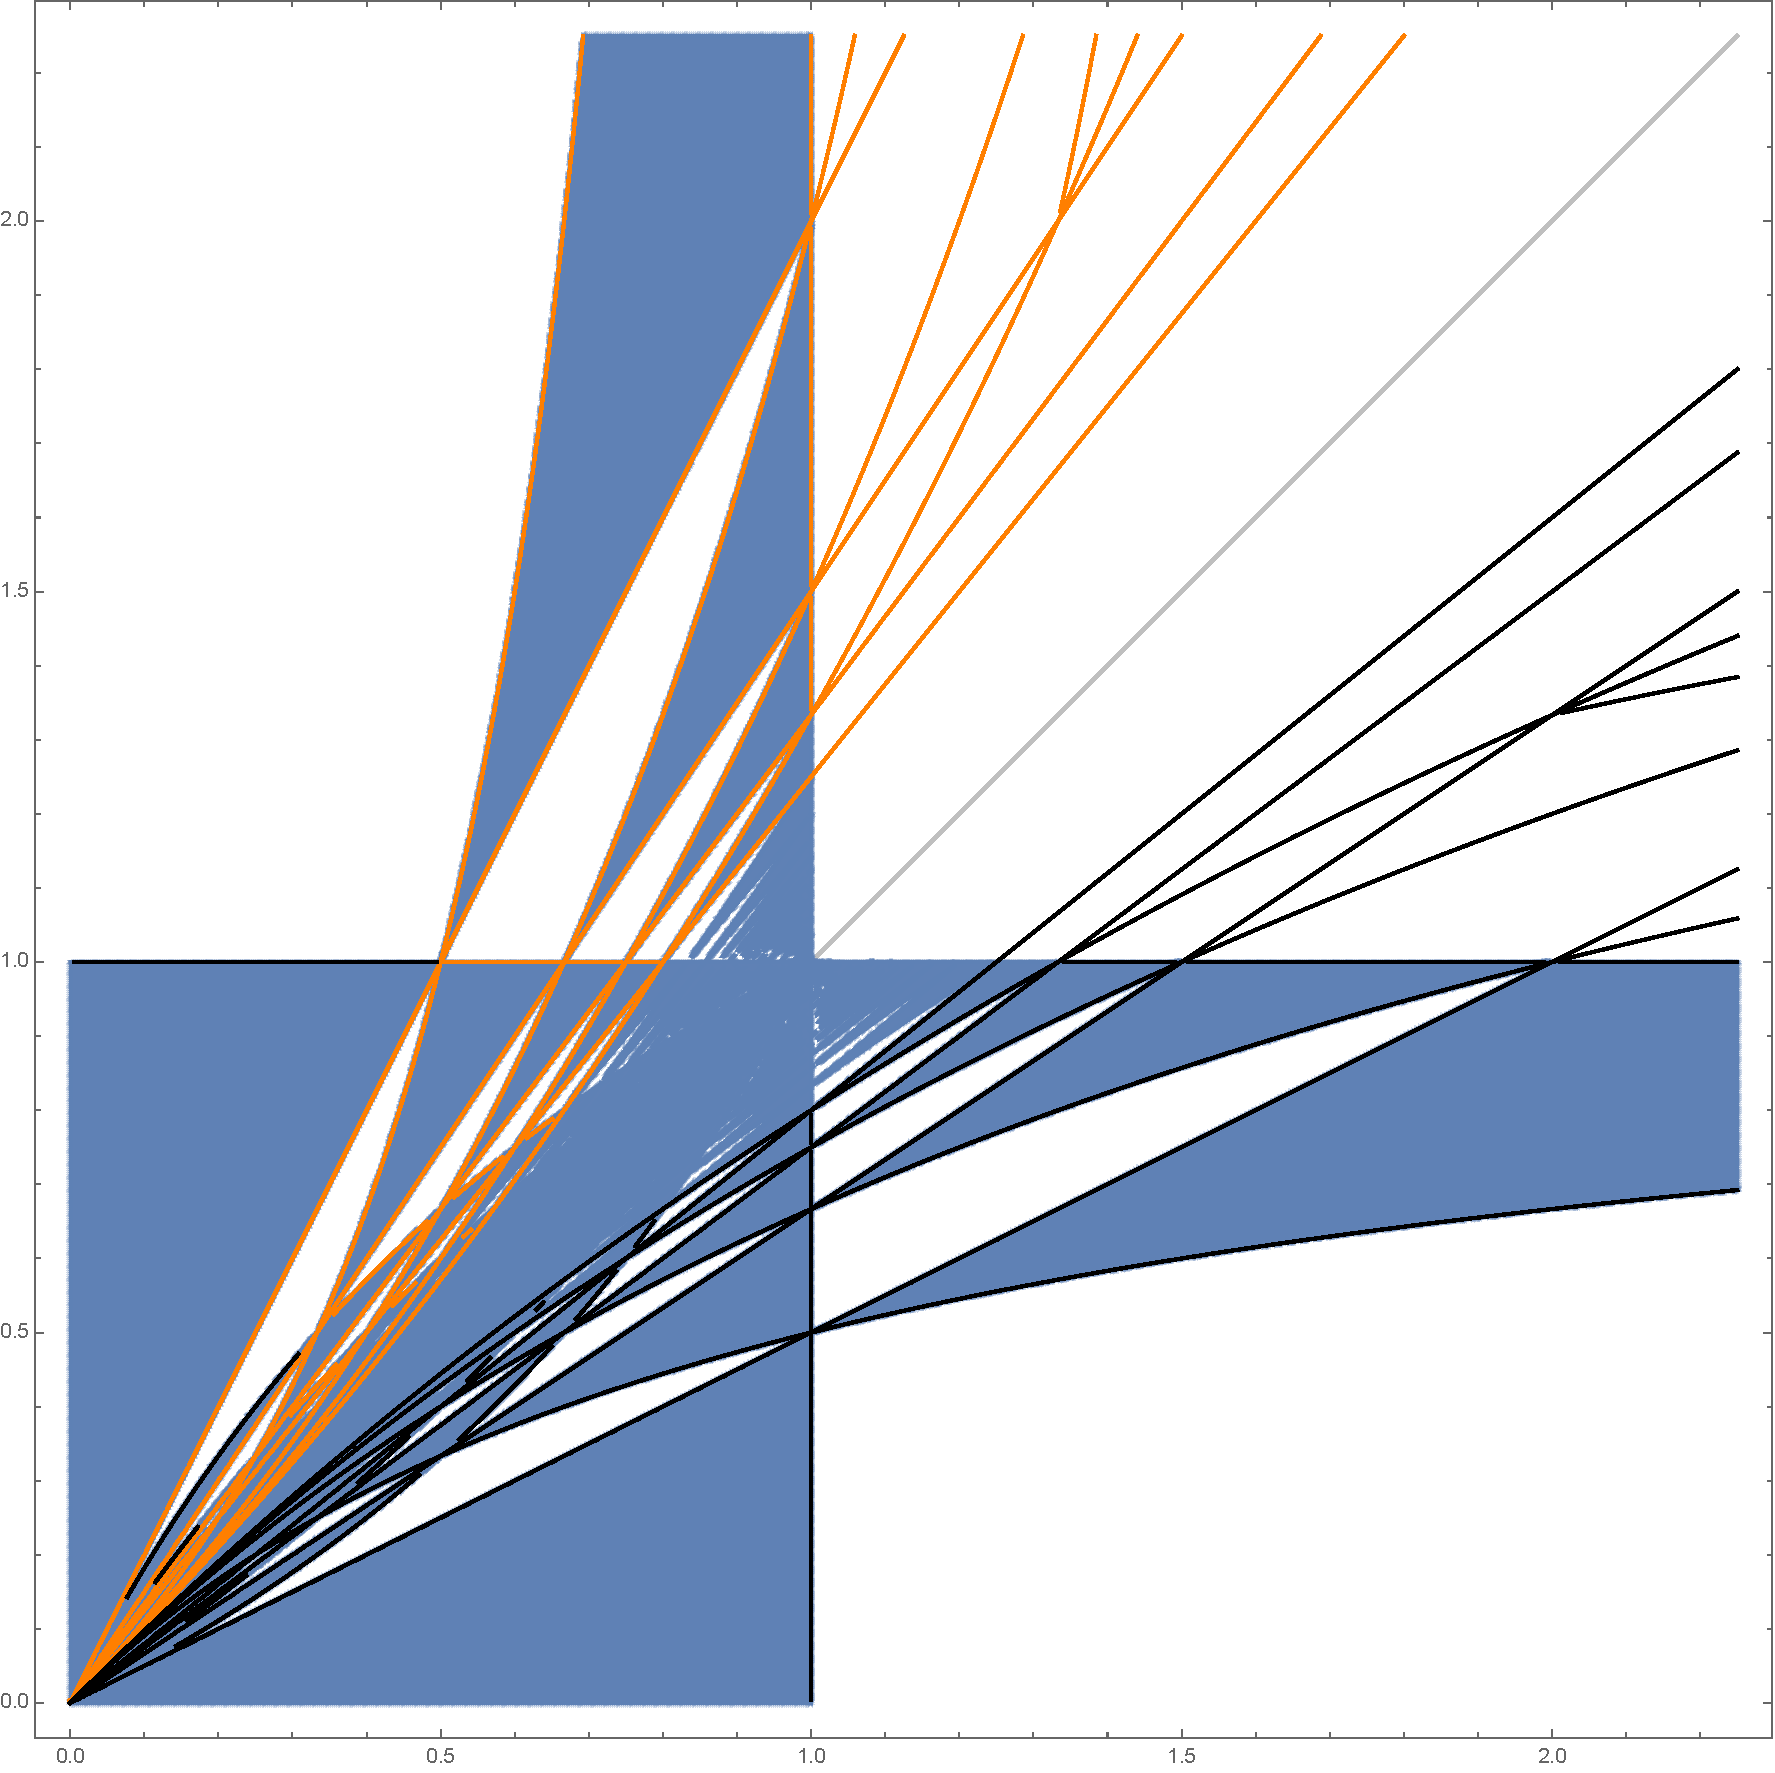
\includegraphics[scale=0.2]{section3_circular/B1_lattice.png}
%\endminipage\hfill
%\minipage{0.5\textwidth}
%\centering
%\includegraphics[scale=0.171]{section3_circular/B1_lattice_labeled.pdf}
%\endminipage\hfill
%\end{figure}
% 
%\qq Точки $A_m$ в белой области имеют k уникальных <<соседей>>, отличающихся на вектор $\left( \gamma / n_1^2,  \gamma / n_2^2 \right)$. 
%
%\qq Для $A_m$ в синей области таких <<соседей>>  на 1 больше.
%
%\end{frame}
%
%\begin{frame}\frametitle{Границы классов $C_k$, $C_{k+1}$. Выражения кривых.}
%\begin{statement}
%Положим $x = \rho_1^2$, $y=\rho_2^2$. Для кривых из семейств $I, II, III$ справедливы следующие уравнения:
%\begin{center}
%\begin{tabular}{|c|c|c|}
%\hline 
%кривая &
%$n_1^2 < n_2^2$  				& 	параметр\\ \hline 
%\hline 
%$I_k$ &
%$y = \dfrac{k-1}{k} x$  				&	$k \geq 2$ \\ \hline 
%$II_m$ &
%$x y = m r_1^2 (x-y)$  		&	$m \geq 1$ \\ \hline 
%$III_m$ &
%$x y = r_1^2 (x-y) \left( m + \left\{\dfrac{x}{x-y}\right\}\right)$  &	$m \geq 0$ \\ \hline 
%\end{tabular}
%\end{center}
%\label{st:curves_formulas}
%\end{statement}
%\qq Преобразуем семейства кривых для простоты. Новая система  координат $(\widetilde{x}, \widetilde{y}) = \left(\dfrac{x y }{(x-y) r_1^2}, \dfrac{x}{x-y}\right)$, где $x=\rho_1^2, y=\rho_2^2$.
%\end{frame}
%
%

\begin{frame}\frametitle{Часть диаграммы $\{ \xi < L_1\}$. Классы $C_k$. Количество поверхностей.}
\begin{figure}[!htb]
\centering
\includegraphics[width=10cm]{section3_circular/two surfaces.png}
\end{figure}
\end{frame}

%\begin{frame}\frametitle{Радиус $r_2$ внешней граничной окружности.}
%\qq Случай $\rho_1 = r_2^2$ тоже накладывает свои кривые, но мы не будем о них говорить. Просто покажем полную диаграмму.
%\begin{figure}[!htb]
%\centering
%\includegraphics[width=8cm]{section3_circular/atoms/branching/C_kPrime_definitions.pdf}
%\end{figure}
%\qq Может быть три поверхности.
%\end{frame}



\begin{frame}\frametitle{Неособые поверхности}
\begin{mytheorem}
Пусть $n_1^2<n_2^2$. В области $\left\{\xi < L_1\right\}$ поверхности $\Xi = \xi =  \const$ являются сферами с $2m$ ручками, если $\rho^2(\xi) \in C_m$ и сферами с $2m-1$ ручками, если $\rho^2(\xi) \in C_m'$.
\end{mytheorem}

\begin{mytheorem}
Пусть $n_1^2>n_2^2$. В области $\left\{\xi < L_1\right\}$ поверхности $\Xi = \xi =  \const$ являются сферами с $2m+1$ ручками, если $\rho^2(\xi) \in C_m$ и сферами с $2m$ ручками, если $\rho^2(\xi) \in C_m'$.
\end{mytheorem}


\qq  Подкласс $C_m'$ соответствует случаю $\rho_1 = r_2^2$ (полное внутреннее отражение на дуге $FG$).
\end{frame}


%\begin{frame}
%\frametitle{Соображения для доказательства.}
%
%\begin{figure}[!htb]
%\centering
%\includegraphics[width=12cm]{section3_circular/big surface step 1.png}
%\end{figure}
%\end{frame}
%
%
%\begin{frame}
%
%\begin{figure}[!htb]
%\minipage{0.5\textwidth}
%\centering
%\includegraphics[width=5cm]{section3_circular/atoms/branching/terminal_min_transformed.pdf}
%\endminipage\hfill
%\minipage{0.5\textwidth}
%\centering
%\includegraphics[width=5cm]{section3_circular/atoms/branching/branching_domain_transformed.pdf}
%\endminipage\hfill
%\end{figure}
%\begin{figure}[!htb]
%\minipage{0.3\textwidth}
%\centering
%\includegraphics[width=5cm]{section3_circular/atoms/branching/terminal_max_transformed.pdf}    
%\endminipage\hfill
%\end{figure}
%
%\end{frame}
%
%\begin{frame}
%\begin{figure}[!htb]
%\centering
%\includegraphics[scale=0.12]{section3_circular/big surface step 2.png}
%    \caption{Склейка большого листа $\widetilde{\Omega}$.}
%\end{figure}
%\qq Остается подсчитать количество чередований правил склейки $r$ и $c$.
%\end{frame}

\begin{frame}\frametitle{Бифуркации.}
\qq Бифуркаций всего две. Обе описаны в тексте. 
\begin{figure}
    \centering
    \includegraphics[width=1\linewidth]{section3_circular/бифуркация Б.png}
\end{figure}
\end{frame}

\begin{frame}\frametitle{Пример бифуркации.}
\qq Пересечение любой синей прямой на большой поверхности проявляется одинаково: исчезают две ручки.

\begin{figure}
    \centering
    \includegraphics[width=0.8\linewidth]{section3_circular/branching bifurcation.png}
    
\end{figure}

\end{frame}

\begin{frame}
\center\LARGE Квантовая задача
\end{frame}


\begin{frame}\frametitle{Области}

\begin{minipage}{\linewidth}
%\begin{center}
\begin{minipage}{0.31\linewidth}
\includegraphics[width=0.95\linewidth]{right3.pdf}

\small Область $A_\delta$, $\phi_0<\pi/2$
\end{minipage}
%\end{center}
%\begin{center}
\begin{minipage}{0.31\linewidth}
\includegraphics[width=0.95\linewidth]{left3.pdf}

\small Область $A_\delta$, $\phi_0>\pi/2$
\end{minipage}
%\end{center}
%\begin{center}
\begin{minipage}{0.31\linewidth}
\includegraphics[width=0.95\linewidth]{up3.pdf}

\small Область $B_\delta$, $\phi_0<\phi_1<\pi/2$
\end{minipage}
%\end{center}
\bigskip
\bigskip\bigskip

\centerline{  Границы областей выделены жирным.}
\centerline{Пунктирами изображены асимптоты гипербол.}
\centerline{ $\phi_0$ и $\phi_1$ -- это углы между соответствующими асимптотами и осью $x$.}
\centerline{Общие фокусы граничных квадрик в точках $(\pm \delta, 0)$.}
\end{minipage}

\end{frame}

\begin{frame}
\begin{mytheorem}[Gongora-T. A., Jose, J.V., Schaffner, S., Tiesinga, P.: {\em Quantum and classical solutions for a free particle in wedge billiards}. Physics Letters A 274(3--4), 117\_122 (2000) 
]
Собственные функции  $\psi_{k,m}(r,\phi)$ и соответствующие уровни энергии $E_{k,m}$ для свободной частицы в круговом секторе размера  $\phi_0$
определены формулами 
\begin{align*}
&\psi_{k, m}(r, \phi) = J_\lambda\left(\frac{\alpha_{\lambda, k}r}{r_0}\right)\sin{\lambda\phi}\notag \\  
&E_{k,m} = \frac{\hbar^2 \alpha_{\lambda, k}^2}{2M r_0^2},
 \qquad k, m \in \mathbb{N},
\end{align*}
где
$\lambda = \frac{\pi m}{\phi_0}$ и $\alpha_{\lambda, k}$ это
$k$-ый нуль функции Бесселя  $J_\lambda(x)$  первого рода.
\end{mytheorem}
\end{frame}


\begin{frame}
\begin{mytheorem}[A]\label{th:A}
В области $A_\delta$ собственными функциями $\psi_{k, m}(\rho, \phi)$ оператора $\hat{H}$ являются
\begin{equation*}
\psi_{k, m}(\rho, \phi) = 
\left[
\begin{array}{ll}
    Ce_\nu(\rho, q) ce_\nu(\phi, q) ,   &    \text{ для нечётных $k \geq 1$}\\
    Se_\nu(\rho, q) se_\nu(\phi, q) ,   &    \text{ для чётных $k \geq 2$}\\
\end{array}
\right.
\end{equation*}
с параметрами
$\nu = \nu_{k,m} = \nu_0+ \delta^2 \frac{\alpha_{\nu_0, m}^2}{4 r_0^2}  \nu_1 + o(\delta^2), \qquad q=q_{k,m} = \dfrac{\varkappa_{k,m}^2 \delta^2}{4},$

где
$\nu_0 = \dfrac{\pi k}{2\phi_0}$,
%\text{\ \  and\  \  }
$\nu_1=\dfrac{\pi k \sin 2\phi_0}{\pi^2 k^2 - 4\phi_0^2}.$

Соответствующими собственными значениями   $\varkappa^2_{k, m}$ являются
\begin{equation*}
\varkappa^2_{k, m} = \dfrac{\alpha_{\nu_0, m}^2}{r_0^2} +
\delta^2 \dfrac{\alpha_{\nu_0, m}^3}{2 r_0^4}\dfrac{\varkappa_1 }{ \left.\frac{\partial J_{\nu_0}(u)}{\partial u}\right|_{u=\alpha_{\nu_0, m}} } + o(\delta^2),
\end{equation*}
где $\varkappa_1 = ...$
\end{mytheorem}
\end{frame} 

\begin{frame}
\begin{mytheorem}[A (продолжение)]

где
\begin{equation*}
    \varkappa_1 = 
    \left[
\begin{array}{ll}
\frac{J_{\nu_0-2}(\alpha_{\nu_0, m})}{4(\nu_0-1)} - \frac{J_{\nu_0+2}(\alpha_{\nu_0, m})}{4(\nu_0+1)} 
  - \nu_1 \left.\frac{\partial J_\nu}{\partial \nu}\right|_{\nu=\nu_0}(\alpha_{\nu_0, m}), \\
  \qquad \qquad \qquad \qquad \qquad \qquad \qquad \qquad \qquad  \text{для нечетных $k\geq 1$ ;} \\[10pt]
\frac{(\nu_0 - 2)J_{\nu_0-2}(\alpha_{\nu_0, m})   }{4\nu_0 (\nu_0-1)} -\\
\qquad - \frac{(\nu_0 + 2)J_{\nu_0+2}(\alpha_{\nu_0, m})}{4\nu_0 (\nu_0+1)}  
- \nu_1 \left.\frac{\partial J_\nu}{\partial \nu}\right|_{\nu = \nu_0}(\alpha_{\nu_0, m}), \\
  \qquad \qquad \qquad \qquad \qquad \qquad \qquad \qquad \qquad  \text{для четных $k \geq 2$}.        
\end{array}
\right.
\end{equation*}

Здесь и далее $\alpha_{\nu_0,m}$ обозначает  $m$-ый нуль функции Бесселя  $J_{\nu_0}(x)$ первого рода.


\end{mytheorem}
\end{frame} 
 


\begin{frame}
\begin{mytheorem}[B]\label{th:B}
В области  $B_\delta$ собственными функциями  $\psi_{k, m}(\rho, \phi)$ и собственными значениями  $\varkappa^2_{k, m}$ оператора  $\hat{H}$ являются
\begin{align*}
&\psi_{k, m}(\rho, \phi) = 
    Se_\nu(\rho, q) \bigl( ce_\nu(\phi_0, q) se_\nu(\phi, q) %{}\notag \\
    %&\qquad\qquad\qquad{}
    -ce_\nu(\phi, q) se_\nu(\phi_0, q) \bigr) ,  
\end{align*}
с параметрами 
\begin{equation*}    
\nu = \nu_{k,m} = \nu_0 +\delta^2 \frac{\alpha_{\nu_0, m}^2}{4 r_0^2} \nu_1 + o(\delta^2), \quad q=q_{k,m} = \frac{\varkappa_{k,m}^2 \delta^2}{4},
\end{equation*}
где
\begin{align*}
& \nu_0 = \frac{\pi k}{\phi_1-\phi_0},\text{\ \ и \ \ }
\nu_1= \frac{\pi k (\sin 2\phi_1 - \sin 2 \phi_0)}{\pi^2k^2-(\phi_1-\phi_0)^2} .
\end{align*}

Соответствующими собственными значениями являются ($\alpha_{\nu_0,m}$ обозначает $m$-ый нуль функции Бесселя $J_{\nu_0}(x)$ первого рода).
$\varkappa_{k, m}^2 = ...$

\end{mytheorem}

\end{frame}  


\begin{frame}
\begin{mytheorem}[B (продолжение)]

\begin{align*}
\varkappa_{k, m}^2 ={}& \frac{\alpha_{\nu_0, m}^2}{r_0^2} +  \delta^2 \frac{\alpha_{\nu_0, m}^3}{2 r_0^4}\frac{1}{ \left.\frac{\partial J_{\nu_0}(u)}{\partial u}\right|_{u=\alpha_{\nu_0, m}} }  
 \biggl(\frac{(\nu_0 - 2)J_{\nu_0-2}(\alpha_{\nu_0, m})   }{4\nu_0 (\nu_0-1)} -
\notag \\ 
&{}- \frac{(\nu_0 + 2)J_{\nu_0+2}(\alpha_{\nu_0, m})}{4\nu_0 (\nu_0+1)} 
- \nu_1 \left.\frac{\partial J_\nu}{\partial \nu}\right|_{\nu = \nu_0}(\alpha_{\nu_0, m})
    \biggr) + o(\delta^2).
\end{align*}

\end{mytheorem}

\end{frame} 

%\begin{frame} 
%
%
%
%\begin{minipage}{\linewidth}
%\begin{center}
%\begin{minipage}{0.3\linewidth}
%\includegraphics[width=0.9\linewidth]{symmetric-34-thick.pdf}
%
%\centerline{\small $\varkappa^2_{3,4}$}
%\end{minipage}
%%\end{center}
%%\begin{center}
%\begin{minipage}{0.3\linewidth}
%\includegraphics[width=0.9\linewidth]{symmetric-35-thick.pdf}
%
%\centerline{\small $\varkappa^2_{3,5}$}
%\end{minipage}
%%\end{center}
%%\begin{center}
%\begin{minipage}{0.3\linewidth}
%\includegraphics[width=0.9\linewidth]{symmetric-44-thick.pdf}
%
%\centerline{\small $\varkappa^2_{4,4}$}
%\end{minipage}
%\end{center}
%
%\centerline{Зависимость $\varkappa^2_{k,m}$ от $\delta$  в области  $A_\delta$ при  $\phi_0=\pi/3$.}
%
%\end{minipage}
%
%\medskip
%\hrule
%\medskip
%
%\begin{minipage}{\linewidth}
%%\begin{center}
%\begin{minipage}{0.3\linewidth}
%\includegraphics[width=0.95\linewidth]{unsymmetric-34-thick.pdf}
%
%\centerline{\small $\varkappa^2_{3,4}$}
%\end{minipage}
%%\end{center}
%%\begin{center}
%\begin{minipage}{0.3\linewidth}
%\includegraphics[width=0.95\linewidth]{unsymmetric-35-thick.pdf}
%
%\centerline{\small $\varkappa^2_{3,5}$}
%\end{minipage}
%%\end{center}
%%\begin{center}
%\begin{minipage}{0.3\linewidth}
%\includegraphics[width=0.95\linewidth]{unsymmetric-44-thick.pdf}
%
%\centerline{\small $\varkappa^2_{4,4}$}
%\end{minipage}
%%\end{center}
%
%
%\centerline{ Зависимость  $\varkappa^2_{k,m}$ от $\delta$
%в области   $B_\delta$ при  $\phi_0=0.3435$, $\phi_1=2.1163$.}
%\centerline{\small  Асимптотика изображена красным пунктиром.
% Численное решение изображено черным.}
%
%
%\end{minipage}
%
% \end{frame} 
%
% \begin{frame} 
%
%
%
%\begin{minipage}{\linewidth}
%\begin{center}
%\begin{minipage}{0.4\linewidth}
%\includegraphics[width=0.8\linewidth]{8.1 together.pdf}
%\end{minipage}
%%\end{center}
%%\begin{center}
%\begin{minipage}{0.4\linewidth}
%\includegraphics[width=0.9\linewidth]{2.4 and 4.3 together.pdf}
%\end{minipage}
%\end{center}
%
%\begin{center}
%\begin{minipage}{0.4\linewidth}
%\includegraphics[width=0.9\linewidth]{5.3 and 3.4 together.pdf}
%\end{minipage}
%\begin{minipage}{0.4\linewidth}
%
%Пример графиков $\varkappa^2_{k,m}$ от $\delta$ в области $A_\delta$ при $\phi_0 > \frac{\pi}{2}$. Полученная асимптотика позволяет определить потенциально вырожденные уровни энергии.
%\end{minipage}
%
%\end{center}
%\end{minipage}
%
%\medskip
%\end{frame} 
%

 
%%%%%%%%%%%%%----------------------- 
\begin{frame} 


Интегрируемость классического бильярда в областях $A_\delta$ и $B_\delta$ следует из существования сохраняющейся величины, а именно, произведения моментов относительно обоих фокусов, который не зависит от полной энергии. 




Соответствующая величина для квантовых бильярдов в областях
 $A_\delta$ и $B_\delta$ может быть определена как
\begin{equation*}
\hat A = -\frac{1}{2}(L_\delta L_{-\delta} + L_{-\delta} L_\delta + \delta^2 \nabla ^2).
\end{equation*}

где  $$\hat L_{\pm \delta} = (x \pm \delta)\frac{\partial}{\partial y} - y\frac{\partial}{\partial x}$$ 
--- угловые моменты относительно фокусов $(x,y) = (\mp \delta, 0)$.


\begin{mytheorem}[C]
\label{th:L}
(a) $\hat A$ коммутирует с  $\hat H$.

(b) Пусть   $\psi(\phi, \rho) = \Phi(\zeta, q, \phi) R(\zeta, q, \rho)$ --- собственная функция оператора $\hat H$. %the operator $\nabla^2$. %, ïðè÷åì $<\psi, \psi>=1$.
%Ïîëîæèì $\Phi_1(a, q, \phi), \Phi_2(a, q, \phi)$ -- íåçàâèñèìûå ðåøåíèÿ óðàâíåíèÿ $\frac{\partial^2}{\partial \phi^2}\Phi + (a - 2q\cos{2\phi})\Phi = 0$, $R_1(a, q, \rho), R_2(a, q, \rho)$ -- íåçàâèñèìûå ðåøåíèÿ óðàâíåíèÿ $\frac{\partial^2}{\partial \rho^2}R - (a - 2q\cosh{2\rho})R = 0$. 
Тогда
$\hat A \psi = \zeta \psi$
\end{mytheorem}

\end{frame} 
